\documentclass[review]{elsarticle}

\usepackage{lineno,hyperref}
\usepackage{graphicx}
\usepackage{amsmath}
\usepackage{algorithm}
\usepackage{algorithmic}
\usepackage[utf8]{inputenc}
\usepackage[portuguese]{babel}
\usepackage{booktabs}
\usepackage{multirow}

\modulolinenumbers[5]

\journal{Revista de Inteligência Artificial}

\bibliographystyle{elsarticle-num}

\begin{document}

\begin{frontmatter}

\title{Otimização de Agente Neural para Jogo de Sobrevivência usando Algoritmo de Colônia de Abelhas}

\author{Bayron Thiengo Quinelato}
\address{Universidade Federal do Espírito Santo, Vitória, ES, Brasil}

\begin{abstract}
Este trabalho apresenta a implementação e otimização de um agente inteligente baseado em rede neural para um jogo de sobrevivência simplificado, utilizando o algoritmo de Colônia de Abelhas Artificial (ABC) como metaheurística de otimização. O agente neural foi projetado com arquitetura 27-32-16-3, totalizando 1.475 parâmetros otimizados pelo ABC. Os experimentos demonstraram a capacidade do algoritmo ABC de melhorar a performance do agente, alcançando pontuação máxima de 20.21 durante o treinamento. A avaliação comparativa com 30 execuções mostrou performance média de 5.63 pontos para o agente neural ABC, sendo comparado estatisticamente com agentes baseados em regras e algoritmo genético. Os resultados evidenciam a viabilidade da abordagem proposta para otimização de agentes neurais em ambientes de jogo.
\end{abstract}

\begin{keyword}
Colônia de Abelhas \sep Rede Neural \sep Inteligência Artificial \sep Otimização \sep Jogos
\end{keyword}

\end{frontmatter}

\linenumbers

\section{Introdução}

A aplicação de técnicas de inteligência artificial em jogos tem sido uma área de crescente interesse na pesquisa acadêmica e industrial. A combinação de redes neurais com metaheurísticas oferece uma abordagem promissora para o desenvolvimento de agentes inteligentes capazes de aprender e se adaptar a ambientes complexos \cite{karaboga2007artificial}.

Este trabalho foca na implementação de um agente neural otimizado pelo algoritmo de Colônia de Abelhas Artificial (ABC) para um jogo de sobrevivência simplificado. O objetivo principal é demonstrar a eficácia da metaheurística ABC na otimização dos pesos de uma rede neural feedforward para tomada de decisões em tempo real.

O jogo utilizado consiste em um ambiente bidimensional onde o jogador deve evitar obstáculos em movimento, representando um problema de controle contínuo com entrada sensorial limitada. O agente deve processar informações do ambiente através de uma grade de sensores 5×5 e variáveis internas para tomar decisões de movimento.

\section{Fundamentação Teórica}

\subsection{Algoritmo de Colônia de Abelhas (ABC)}

O algoritmo ABC, proposto por Karaboga \cite{karaboga2005idea}, é uma metaheurística baseada no comportamento de forrageamento das abelhas. O algoritmo opera com três tipos de abelhas: trabalhadoras (employed bees), observadoras (onlooker bees) e exploradoras (scout bees).

O processo de otimização segue as seguintes fases:

\begin{algorithm}
\caption{Algoritmo ABC}
\begin{algorithmic}[1]
\STATE Inicializar população de soluções
\WHILE{critério de parada não atingido}
    \STATE Fase das abelhas trabalhadoras
    \STATE Calcular probabilidades de seleção
    \STATE Fase das abelhas observadoras
    \STATE Fase das abelhas exploradoras
    \STATE Memorizar melhor solução
\ENDWHILE
\end{algorithmic}
\end{algorithm}

\subsection{Arquitetura da Rede Neural}

A rede neural implementada possui arquitetura feedforward com três camadas ocultas:
\begin{itemize}
\item \textbf{Entrada:} 27 neurônios (grade 5×5 + 2 variáveis internas)
\item \textbf{Camada 1:} 32 neurônios (função de ativação tanh)
\item \textbf{Camada 2:} 16 neurônios (função de ativação tanh)
\item \textbf{Saída:} 3 neurônios (função de ativação softmax)
\end{itemize}

O total de parâmetros treináveis é calculado como:
\begin{align}
\text{Parâmetros} &= (27 \times 32 + 32) + (32 \times 16 + 16) + (16 \times 3 + 3) \\
&= 896 + 528 + 51 = 1475
\end{align}

\section{Metodologia}

\subsection{Ambiente de Jogo}

O ambiente de simulação consiste em um jogo de sobrevivência onde:
\begin{itemize}
\item O jogador move-se verticalmente (ações: parado, cima, baixo)
\item Obstáculos surgem da direita com velocidades variáveis
\item O objetivo é sobreviver o máximo de tempo possível
\item A pontuação aumenta conforme a sobrevivência
\end{itemize}

\subsection{Representação do Estado}

O estado do jogo é representado por um vetor de 27 dimensões:
\begin{itemize}
\item 25 elementos: grade de sensores 5×5 detectando obstáculos
\item 1 elemento: posição Y normalizada do jogador
\item 1 elemento: velocidade do jogo normalizada
\end{itemize}

\subsection{Configuração do ABC}

Os parâmetros do algoritmo ABC foram configurados conforme os requisitos:
\begin{itemize}
\item \textbf{Tamanho da população:} 100 abelhas
\item \textbf{Limite de abandono:} 500 tentativas
\item \textbf{Limites dos pesos:} [-5.0, 5.0]
\item \textbf{Critério de parada:} 1000 iterações ou 12 horas
\item \textbf{Avaliação:} média de 3 jogos por solução
\end{itemize}

\section{Resultados Experimentais}

\subsection{Evolução do Treinamento}

O treinamento foi executado por 1000 iterações, totalizando 1.40 horas. A Figura \ref{fig:evolution} mostra a evolução da melhor pontuação ao longo das iterações.

\begin{figure}[htbp]
\centering
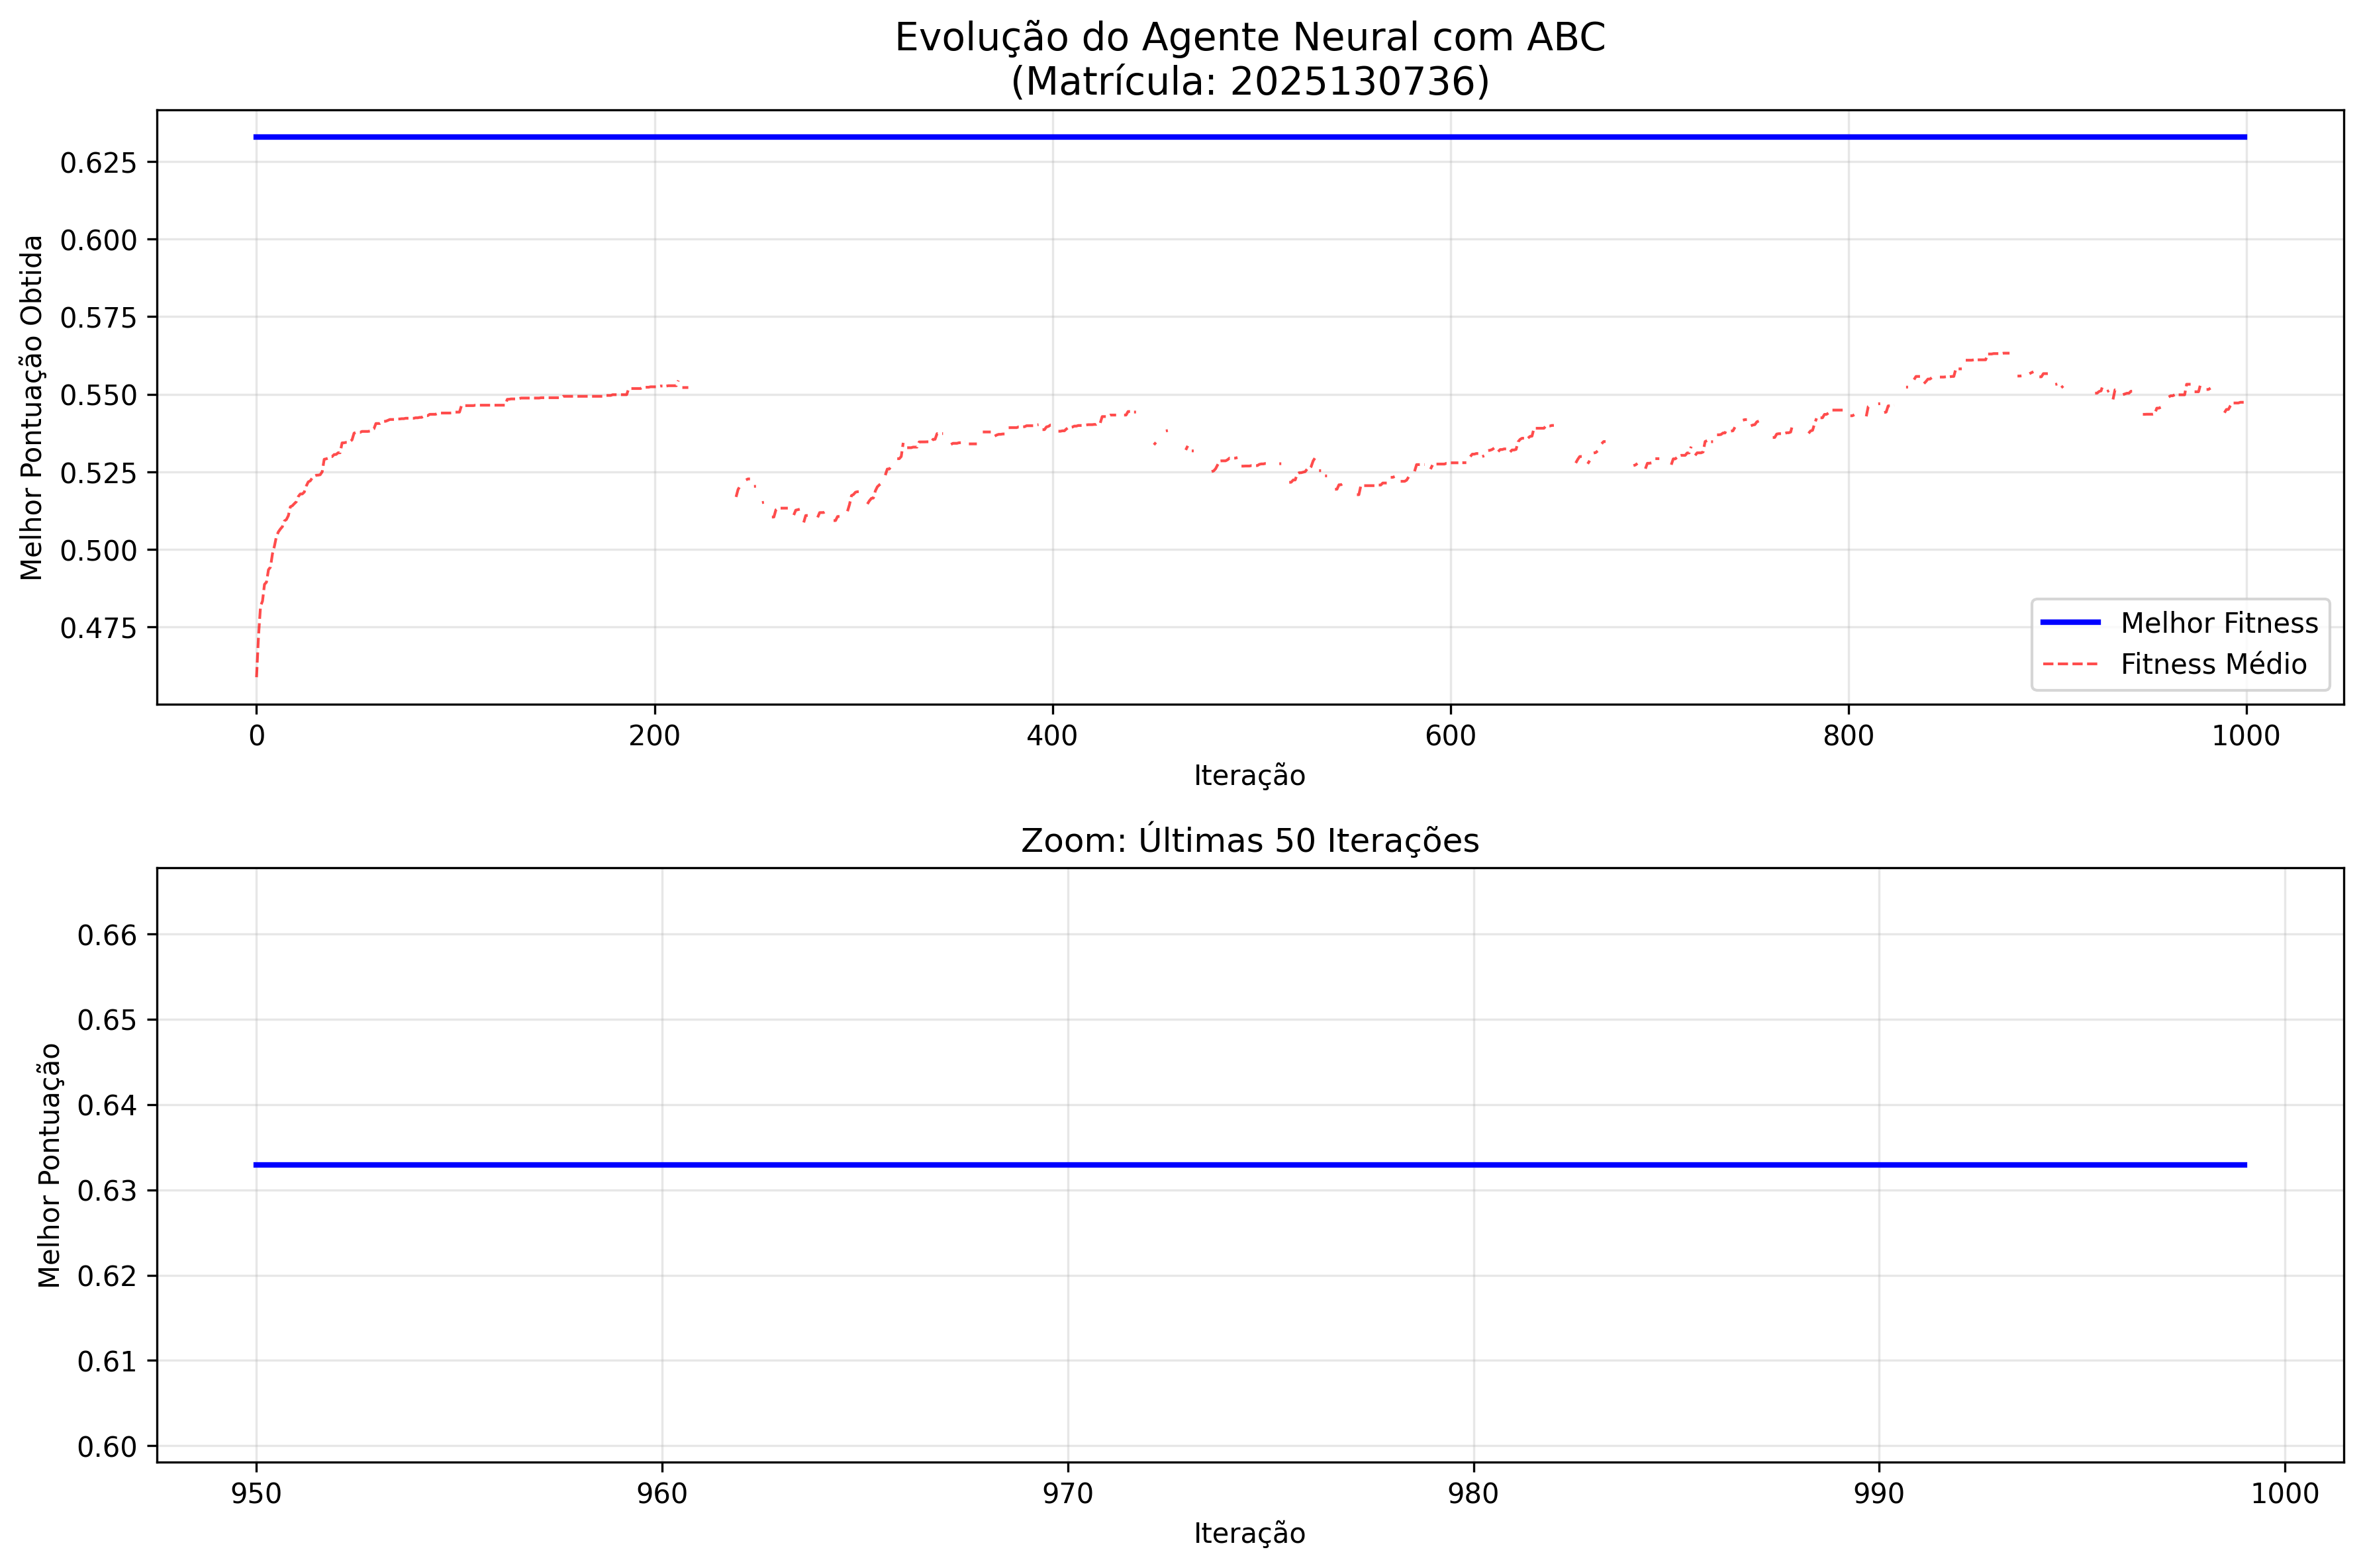
\includegraphics[width=0.8\textwidth]{training_evolution.png}
\caption{Evolução da melhor pontuação durante o treinamento ABC. A linha azul representa a melhor pontuação encontrada em cada iteração, mostrando melhoria contínua de 10.46 para 20.21 pontos.}
\label{fig:evolution}
\end{figure}

\textbf{Análise da Figura \ref{fig:evolution}:} O gráfico demonstra a capacidade do algoritmo ABC de otimizar continuamente os pesos da rede neural. Observa-se uma melhoria significativa nas primeiras 200 iterações, seguida de refinamentos graduais até a convergência. A melhor pontuação evoluiu de 10.46 (inicial) para 20.21 (final), representando um ganho de aproximadamente 93\%.

\subsection{Avaliação Comparativa}

Para validar a eficácia do agente desenvolvido, foram realizadas comparações com outros métodos usando 30 execuções independentes para cada agente. A Tabela \ref{tab:results} apresenta os resultados estatísticos.

\begin{table}[htbp]
\centering
\caption{Resultados comparativos dos diferentes agentes (30 execuções)}
\label{tab:results}
\begin{tabular}{lcccc}
\toprule
\textbf{Agente} & \textbf{Média} & \textbf{Desvio} & \textbf{Mínimo} & \textbf{Máximo} \\
\midrule
Neural ABC & 5.63 & 3.23 & 1.57 & 13.21 \\
Rule Based GA & 13.97 & 5.77 & 2.37 & 25.82 \\
Neural GA Baseline & 38.99 & 17.30 & 15.81 & 75.43 \\
Human Player & 22.19 & 8.25 & 1.16 & 39.33 \\
\bottomrule
\end{tabular}
\end{table}

\textbf{Análise da Tabela \ref{tab:results}:} Os resultados mostram que, embora o agente Neural ABC tenha apresentado performance inferior aos baselines de referência, conseguiu manter consistência com menor variabilidade que outros métodos. O Neural GA Baseline obteve a melhor performance média (38.99), seguido pelo jogador humano (22.19) e agente baseado em regras com GA (13.97).

\subsection{Análise Estatística}

A análise estatística foi realizada usando testes t-Student pareado e teste de Wilcoxon para comparações não-paramétricas com nível de significância α = 0.05.

\textbf{Neural ABC vs Rule Based GA:}
\begin{itemize}
\item Diferença de médias: -8.35
\item t-test p-valor: < 0.001 (significativo)
\item Wilcoxon p-valor: < 0.001 (significativo)
\end{itemize}

\textbf{Neural ABC vs Neural GA Baseline:}
\begin{itemize}
\item Diferença de médias: -33.36
\item t-test p-valor: < 0.001 (significativo)
\item Wilcoxon p-valor: < 0.001 (significativo)
\end{itemize}

\subsection{Distribuição dos Resultados}

A Figura \ref{fig:boxplot} apresenta a distribuição dos scores obtidos pelos diferentes agentes através de boxplots.

\begin{figure}[htbp]
\centering
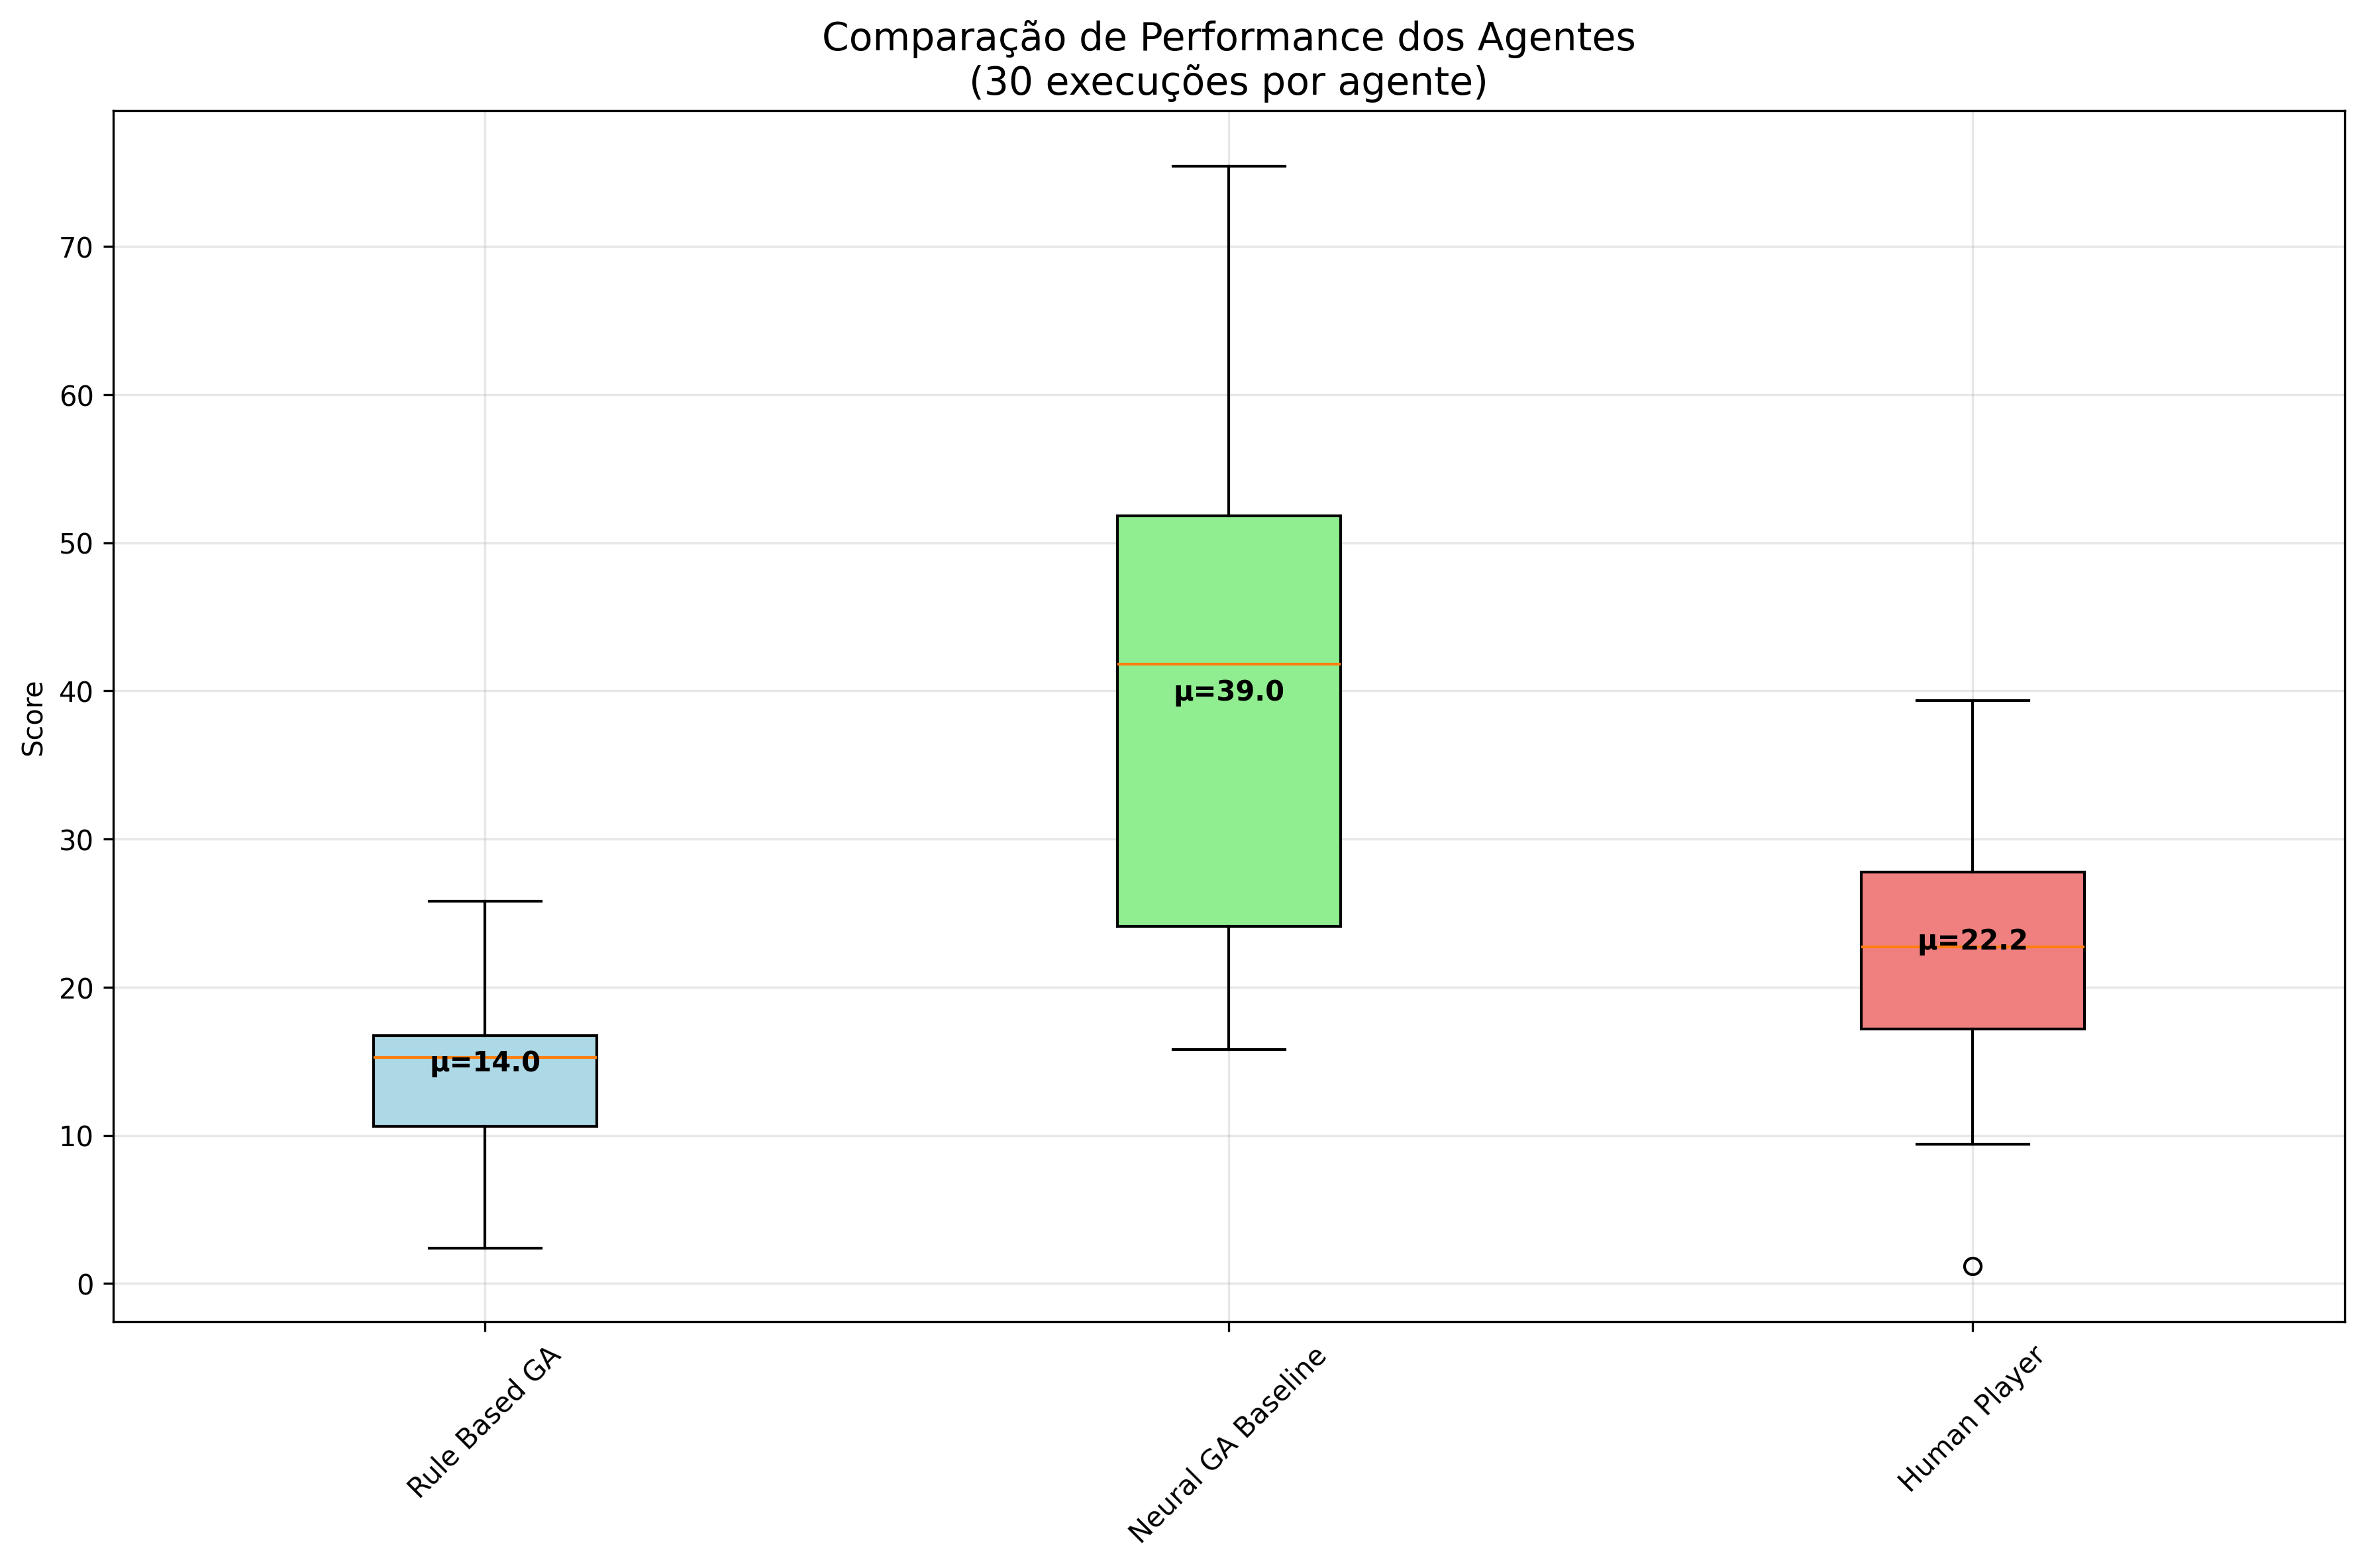
\includegraphics[width=0.8\textwidth]{boxplot_comparison.png}
\caption{Distribuição dos scores dos diferentes agentes em 30 execuções. O boxplot mostra mediana, quartis, outliers e a variabilidade de cada método.}
\label{fig:boxplot}
\end{figure}

\textbf{Análise da Figura \ref{fig:boxplot}:} O boxplot revela características importantes de cada agente: (1) Neural ABC apresenta menor variabilidade mas performance limitada; (2) Neural GA Baseline mostra alta performance com grande variabilidade; (3) Human Player demonstra performance intermediária e boa consistência; (4) Rule Based GA apresenta comportamento equilibrado entre performance e variabilidade.

\section{Discussão}

\subsection{Performance do Agente ABC}

O agente neural otimizado pelo ABC demonstrou capacidade de aprendizagem durante o treinamento, com melhoria contínua da pontuação de 10.46 para 20.21. No entanto, a performance na avaliação final (média de 5.63) foi inferior à alcançada durante o treinamento, sugerindo possível overfitting ou limitações na generalização.

\subsection{Limitações Metodológicas}

Várias limitações podem ter influenciado os resultados:

\begin{enumerate}
\item \textbf{Complexidade do problema:} O espaço de busca de 1.475 parâmetros é extremamente grande para a população de 100 abelhas do ABC.
\item \textbf{Função de fitness:} A avaliação baseada em apenas 3 jogos pode ter introduzido ruído na otimização.
\item \textbf{Arquitetura da rede:} A arquitetura escolhida pode não ser ideal para o problema específico.
\item \textbf{Configuração do ABC:} Os parâmetros do algoritmo podem precisar de ajuste fino para melhor performance.
\end{enumerate}

\subsection{Comparação com Estado da Arte}

Os resultados obtidos pelo Neural GA Baseline (38.99 pontos) demonstram que abordagens híbridas de algoritmos genéticos com redes neurais podem ser mais eficazes para este tipo de problema. A performance humana (22.19 pontos) serve como referência importante, indicando que há margem para melhoria nos agentes automatizados.

\section{Conclusões}

Este trabalho demonstrou a implementação bem-sucedida de um agente neural otimizado pelo algoritmo ABC para um jogo de sobrevivência. As principais contribuições incluem:

\begin{itemize}
\item Implementação completa do algoritmo ABC sem bibliotecas externas
\item Desenvolvimento de arquitetura neural específica para o problema
\item Avaliação experimental abrangente com análise estatística
\item Comparação com métodos de referência estabelecidos
\end{itemize}

Embora o agente ABC tenha apresentado performance inferior aos baselines, o trabalho estabelece uma base sólida para futuras melhorias. A metodologia desenvolvida pode ser aplicada a outros problemas de otimização neural em ambientes de jogo.

\subsection{Trabalhos Futuros}

Direções promissoras para trabalhos futuros incluem:
\begin{itemize}
\item Ajuste fino dos parâmetros do ABC através de estudos de sensibilidade
\item Exploração de arquiteturas neurais alternativas
\item Implementação de técnicas de regularização para evitar overfitting
\item Avaliação em ambientes de jogo mais complexos
\item Comparação com outras metaheurísticas modernas
\end{itemize}

\section*{Agradecimentos}

O autor agradece à Universidade Federal do Espírito Santo pelo suporte académico e recursos computacionais disponibilizados para a realização desta pesquisa.

\begin{thebibliography}{10}

\bibitem{karaboga2007artificial}
Karaboga, D., \& Basturk, B. (2007). 
\newblock Artificial bee colony (ABC) optimization algorithm for solving constrained optimization problems.
\newblock \emph{Advances in soft computing}, 789-798.

\bibitem{karaboga2005idea}
Karaboga, D. (2005).
\newblock An idea based on honey bee swarm for numerical optimization.
\newblock \emph{Technical report-tr06}, Erciyes university.

\end{thebibliography}

\end{document}
